%%%%%%%%%%%%%%%%%%%%%%%%%%%%%%%%%%%%%%%%%
% Beamer Presentation
% LaTeX Template
% Version 1.0 (10/11/12)
%
% This template has been downloaded from:
% http://www.LaTeXTemplates.com
%
% License:
% CC BY-NC-SA 3.0 (http://creativecommons.org/licenses/by-nc-sa/3.0/)
%
%%%%%%%%%%%%%%%%%%%%%%%%%%%%%%%%%%%%%%%%%

%----------------------------------------------------------------------------------------
%	PACKAGES AND THEMES
%----------------------------------------------------------------------------------------

\documentclass{beamer}

\usepackage{ctex}

\mode<presentation> {
	
	% The Beamer class comes with a number of default slide themes
	% which change the colors and layouts of slides. Below this is a list
	% of all the themes, uncomment each in turn to see what they look like.
	
	%\usetheme{default}
	%\usetheme{AnnArbor}
	%\usetheme{Antibes}
	%\usetheme{Bergen}
	\usetheme{Berkeley}
	%\usetheme{Berlin}
	%\usetheme{Boadilla}
	%\usetheme{CambridgeUS}
	%\usetheme{Copenhagen}
	%\usetheme{Darmstadt}
	%\usetheme{Dresden}
	%\usetheme{Frankfurt}
	%\usetheme{Goettingen}
	%\usetheme{Hannover}
	%\usetheme{Ilmenau}
	%\usetheme{JuanLesPins}
	%\usetheme{Luebeck}
	%\usetheme{Madrid}
	%\usetheme{Malmoe}
	%\usetheme{Marburg}
	%\usetheme{Montpellier}
	%\usetheme{PaloAlto}
	%\usetheme{Pittsburgh}
	%\usetheme{Rochester}
	%\usetheme{Singapore}
	%\usetheme{Szeged}
	%\usetheme{Warsaw}
	
	% As well as themes, the Beamer class has a number of color themes
	% for any slide theme. Uncomment each of these in turn to see how it
	% changes the colors of your current slide theme.
	
	%\usecolortheme{albatross}
	%\usecolortheme{beaver}
	%\usecolortheme{beetle}
	%\usecolortheme{crane}
	%\usecolortheme{dolphin}
	%\usecolortheme{dove}
	%\usecolortheme{fly}
	%\usecolortheme{lily}
	%\usecolortheme{orchid}
	%\usecolortheme{rose}
	%\usecolortheme{seagull}
	%\usecolortheme{seahorse}
	%\usecolortheme{whale}
	%\usecolortheme{wolverine}
	
	%\setbeamertemplate{footline} % To remove the footer line in all slides uncomment this line
	%\setbeamertemplate{footline}[page number] % To replace the footer line in all slides with a simple slide count uncomment this line
	
	%\setbeamertemplate{navigation symbols}{} % To remove the navigation symbols from the bottom of all slides uncomment this line
}

\usepackage{graphicx} % Allows including images
\usepackage{booktabs} % Allows the use of \toprule, \midrule and \bottomrule in tables

%----------------------------------------------------------------------------------------
%	TITLE PAGE
%----------------------------------------------------------------------------------------

\title[Cupt2020]{Cupt2020 - 13组} % The short title appears at the bottom of every slide, the full title is only on the title page

\author{13组} % Your name
\institute[UCLA] % Your institution as it will appear on the bottom of every slide, may be shorthand to save space
{
	University of California \\ % Your institution for the title page
	\medskip
	\textit{annan@shanghaitech.edu.cn} % Your email address
}

\begin{document}
	
	\begin{frame}
		\titlepage % Print the title page as the first slide
	\end{frame}
	
	\begin{frame}
		\frametitle{目录} % Table of contents slide, comment this block out to remove it
		\tableofcontents % Throughout your presentation, if you choose to use \section{} and \subsection{} commands, these will automatically be printed on this slide as an overview of your presentation
	\end{frame}
	
	%----------------------------------------------------------------------------------------
	%	PRESENTATION SLIDES
	%----------------------------------------------------------------------------------------
	
	%------------------------------------------------
	\section{\fangsong{实验介绍}} % Sections can be created in order to organize your presentation into discrete blocks, all sections and subsections are automatically printed in the table of contents as an overview of the talk
	%------------------------------------------------
	\subsection{\fangsong{第九题简介}}
	\begin{frame}
		\frametitle{\fangsong{第九题简介}}
			Under certain circumstances, the 'flea' of a magnetic stirrer can rise up and levitate stably in a viscous fluid during stirring. Investigate the origins of the dynamic stabilization of the 'flea' and how it depends on the relevant parameters.
			\\\fangsong{在一定条件下,磁力搅拌器的“搅拌子”在搅拌过程中可以在粘性流体中稳定地上升和悬浮。研究“搅拌子”动态稳定的原因及其如何依赖于相关参数。}
	\end{frame}
	
	%------------------------------------------------
	\subsection{\fangsong{基本量测量}}
	\begin{frame}
		\frametitle{\fangsong{基本量测量}}
		\begin{itemize}
			\item\heiti{{实验仪器和材料}}\\
			\fangsong{条形搅拌子,甘油,水,量筒(100ml,1000ml),磁铁,结晶皿,滴管,小钢珠,电子天平,秒表,照相机,LED灯}
			\item\heiti{{实验过程}}\\
			\fangsong{a) 流体密度的测量\\
				b) 流体粘滞系数的测量\\
				由于实验条件的限制,我们没有合适的测量流体粘滞系数的仪器,采用落球法进行测量。\\}
		\end{itemize}
		\begin{figure}[H]
			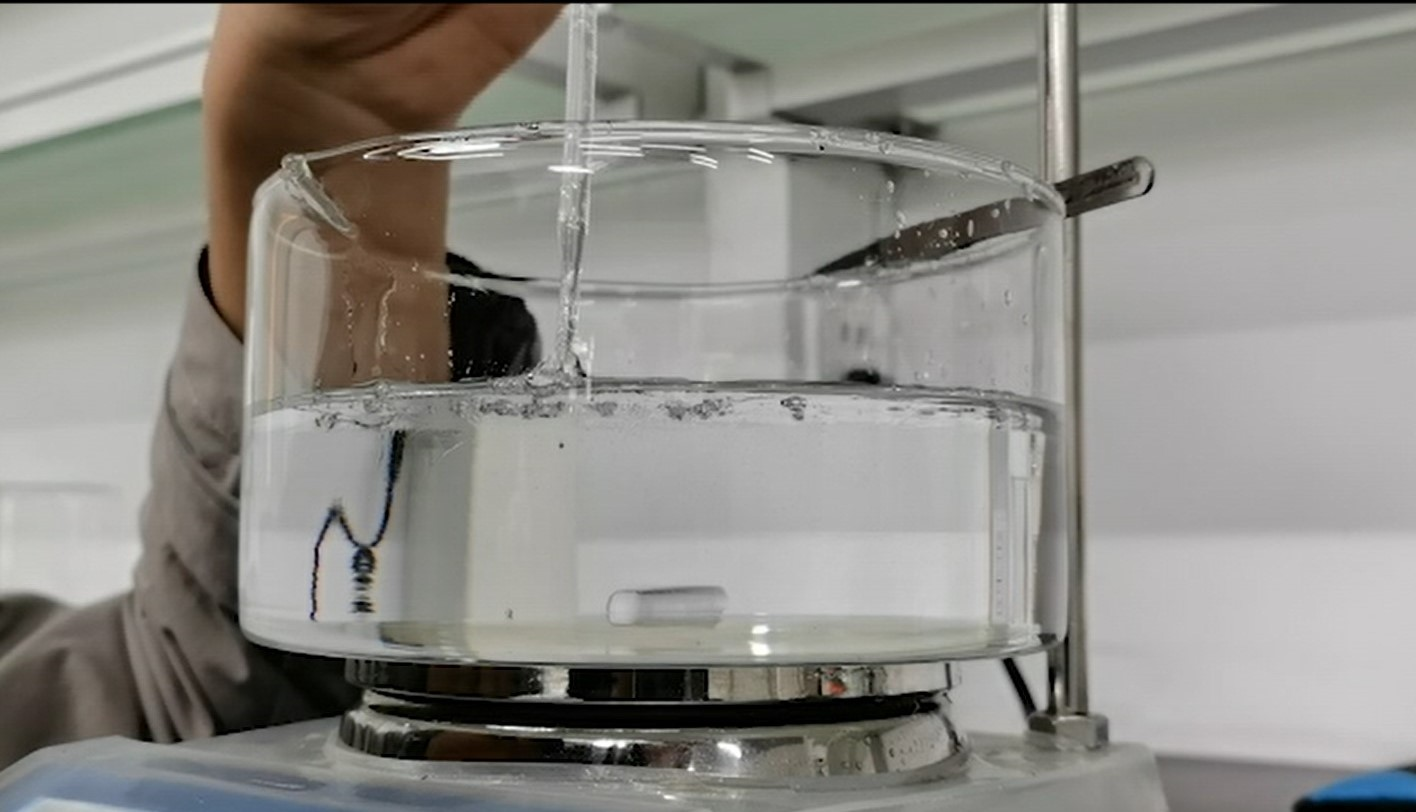
\includegraphics[width=0.4\textwidth]{落球法}
			\caption{\fangsong{落球法测量流体粘滞系数}}
		\end{figure}
	\end{frame}

	\begin{frame}
		\frametitle{\fangsong{基本量测量}}
		\begin{itemize}
			\item\heiti{{实验过程}}\\
			\fangsong{c) 流体密度的测量\\
				将磁子放在1000ml量筒中,量筒中盛放有一定量的实验用的甘油水溶液。在量筒外使用两块磁铁,将磁子吸至液体表面并控制磁子在量筒中保持水平。然后释放磁铁,使之自然下落。使用固定的照相机记录整个过程,使用tracker追踪磁子。	
			}
		\end{itemize}
		\begin{figure}[H]
			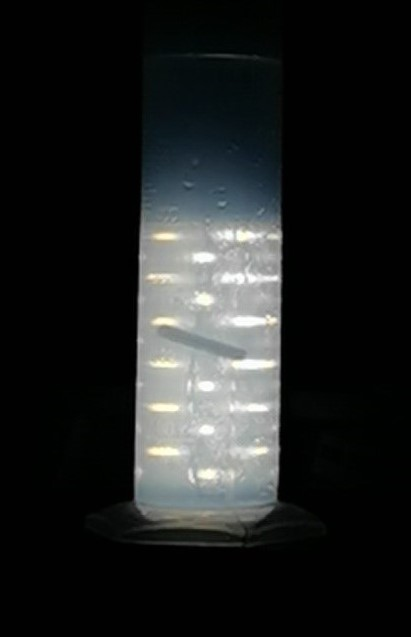
\includegraphics[width=0.2\textwidth]{磁子收尾速度的测量}
			\caption{\fangsong{磁子收尾速度的测量}}
		\end{figure}
	\end{frame}
	
	\subsection{\fangsong{定量分析}}
	\begin{frame}
		\frametitle{\fangsong{定量分析}}
		\begin{itemize}
			\item\heiti{{实验仪器和材料}}\\
			\fangsong{磁力搅拌器,条形搅拌子,甘油,水,结晶皿,玻璃杯,秒表,照相机,记号笔}
		\end{itemize}
	\end{frame}
	
	\begin{frame}
		\frametitle{\fangsong{定量分析}}
		\begin{itemize}
			\item\heiti{{实验过程}}\\
			\fangsong{a) 磁子高度与搅拌器转速的关系\\
				在玻璃杯内倒入甘油的水溶液,并在中央放入磁子。将搅拌器转速调至最高转速(1500r/min)后打开,使搅拌器转速从0开始随时间不断增加。使用固定的照相机记录全过程,使用tracker追踪磁子。
			}
		\end{itemize}
		\begin{figure}[H]
			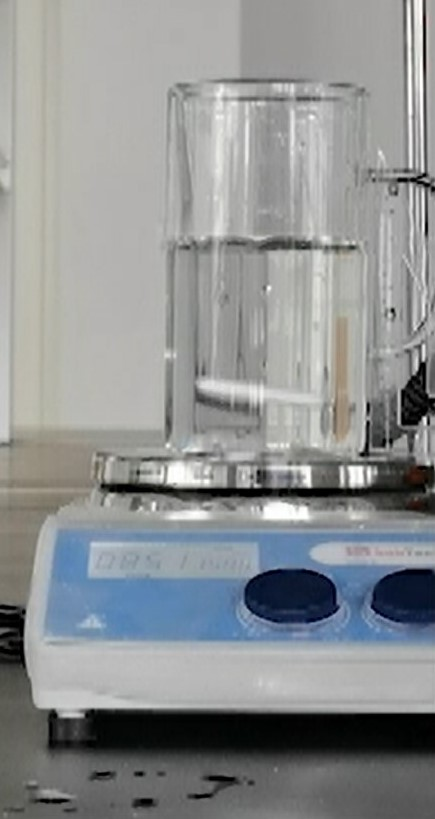
\includegraphics[width=0.2\textwidth]{磁子高度与搅拌器转速定量关系测量的实验过程}
			\caption{\fangsong{磁子高度与搅拌器转速定量关系测量的实验过程}}
		\end{figure}
	\end{frame}
	
	\begin{frame}
		\frametitle{\fangsong{定量分析}}
		\begin{itemize}
			\item\heiti{{实验过程}}\\
			\fangsong{b) 磁子高度变化与时间的关系\\
				在磁子外套焊有小锡球的小环以便tracker准确追踪,将其放在倒有甘油水溶液的结晶皿中央。调节磁力搅拌器的转速分别为1000、1100、1200、1300、1400、1500r/min,待磁子稳定后使用固定的照相机慢镜头拍摄,使用tracker追踪磁子下方的小锡球。
			}
		\end{itemize}
		\begin{figure}[H]
			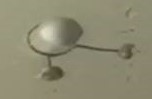
\includegraphics[width=0.4\textwidth]{套有小环的磁子}
			\caption{\fangsong{套有小环的磁子}}
		\end{figure}
	\end{frame}

	\begin{frame}
		\frametitle{\fangsong{定量分析}}
		\begin{itemize}
			\item\heiti{{实验过程}}\\
			\fangsong{c) 磁子旋转的角度与时间的关系\\
				在磁子一端用黑色记号笔标记以便tracker准确追踪,将其放在倒有甘油水溶液的结晶皿中央。调节磁力搅拌器的转速分别为1100、1200、1300、1400、1500r/min,待磁子稳定后使用固定的照相机慢镜头拍摄,使用tracker追踪磁子的一端。
			}
		\end{itemize}
		\begin{figure}[H]
			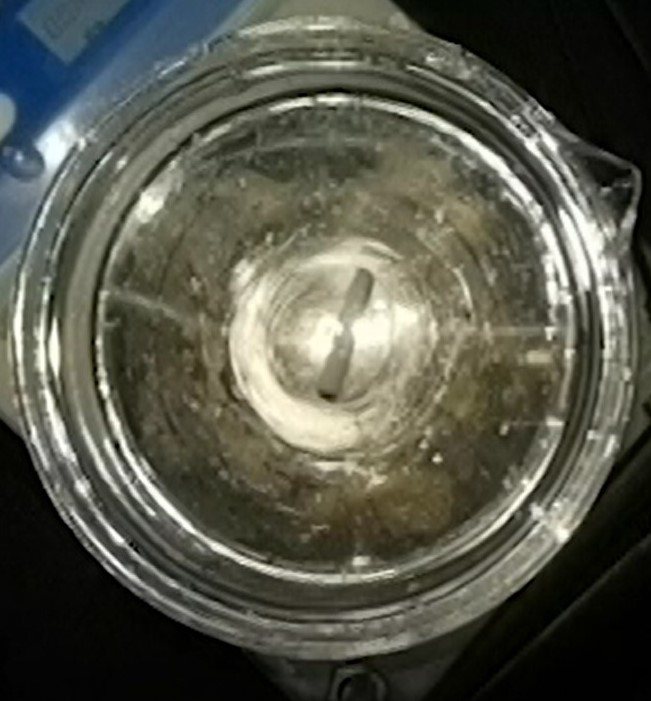
\includegraphics[width=0.3\textwidth]{磁子旋转的角度与时间定量关系测量的实验过程}
			\caption{\fangsong{磁子旋转的角度与时间定量关系测量的实验过程}}
		\end{figure}
	\end{frame}

	
	%------------------------------------------------
	\subsection{\fangsong{实验结果}}
	\begin{frame}
		\frametitle{\fangsong{实验结果}}
		
	\end{frame}
	
	%------------------------------------------------
	\section{\fangsong{理论部分}}
	%------------------------------------------------
	
	
	
	\section{\fangsong{数据分析}}
	\section{\fangsong{结论}}
	%------------------------------------------------
	
	\begin{frame}
		\Huge{\centerline{\fangsong{砍人大赛:街头霸王}}}
	\end{frame}
	
	%----------------------------------------------------------------------------------------
	
\end{document} 
